\documentclass[../main.tex]{subfiles}
\graphicspath{{\subfix{../images/}}}
\begin{document}
\section*{Term 2 Week 8}

\begin{enumerate}[itemsep=1cm]
    \item 
    \(\int \sqrt{1-x}.\sqrt{x+3}\,dx\)

    \(\int \sqrt{-x^2-2x+3}\,dx\)

    Completing the square:

    \(\int \sqrt{-(x^2+2x)+3}\,dx\)

    \(\int \sqrt{-((x+1)^2-1)+3}\,dx\)

    \(\int \sqrt{4-(x+1)^2}\,dx\)

    \begin{figure}[h]
        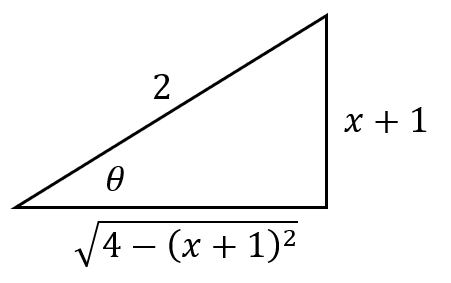
\includegraphics[width=0.25\linewidth]{../images/t2w8q1a.png}
    \end{figure}
    \(\sin{\theta}=\frac{x+1}{2}\\
    x+1=2\sin{\theta}\\
    dx=2\cos{\theta}\,d\theta\)

    Substitute into the integral:\\
    \(\int \sqrt{4-(2\sin{\theta})^2}.2\cos{\theta}\,d\theta\)

    \(\int \sqrt{4-4\sin^2{\theta}}.2\cos{\theta}\,d\theta\)

    \(\int \sqrt{4(1-\sin^2{\theta})}.2\cos{\theta}\,d\theta\)

    \(\int \sqrt{4\cos^2{\theta}}.2\cos{\theta}\,d\theta\)

    \(\int 2\cos{\theta}.2\cos{\theta}\,d\theta\)

    \(4\int \cos^2{\theta}\,d\theta\)

    Using cosine double angle rule, \(\cos{2\theta}=2\cos^2{\theta}-1\), we know \(\cos^2{\theta}=\frac{1}{2}(\cos{2\theta}+1)\)

    \(2\int (\cos{2\theta}+1)\,d\theta=2(\frac{\sin{2\theta}}{2}+\theta)+c=\sin{2\theta}+2\theta+c\)

    Use the sine double angle rule:
    \(2\sin{\theta}\cos{\theta}+2\theta+c\)

    Use the triangle to rewrite in terms of \(x\):
    \(\sin{\theta}=\frac{x+1}{2}, \cos{\theta}=\frac{\sqrt{4-(x+1)^2}}{2}, \theta=\sin^{-1}{\frac{x+1}{2}}\)

    \(\int \sqrt{1-x}.\sqrt{x+3}\,dx=2\frac{x+1}{2}\times \frac{\sqrt{4-(x+1)^2}}{2}+2\times \sin^{-1}{(\frac{x+1}{2})}+c\)

    \(=\frac{(x+1)\sqrt{4-(x+1)^2}}{2}+2\sin^{-1}{(\frac{x+1}{2})}+c\)
    
    \item 
    $
    \sin{x}\cos{y}=\frac{1}{4}\\
    \sin{y}\cos{x}=\frac{3}{4}
    $

    Subtract the equations and use the compound angles formula for sine:\\
    $
    \sin{y}\cos{x}-\sin{x}\cos{y}=\frac{1}{2}\\
    \sin{(y-x)}=\frac{1}{2}\\
    $
    We can solve this using the sine general formula:\\
    Remembering \(\sin^{-1}{(\frac{1}{2})}=\frac{\pi}{6}\)

    \(y-x=n\pi + (-1)^n\times \frac{\pi}{6}\\
    n=0 \Rightarrow : y-x = \frac{\pi}{6}\\
    n=1 \Rightarrow : y-x = \frac{5\pi}{6}\\
    n=-1 \Rightarrow : y-x = \frac{-7\pi}{6}\\
    n=-2 \Rightarrow : y-x = \frac{-11\pi}{6}\\
    \)
    
    Add the equations and use the compound angles formula for sine again:\\
    \(\sin{y}\cos{x}+\sin{x}\cos{y}=1\\
    \sin{(x+y)}=1\)

    We know that \(\sin^{-1}{(1)}=\frac{\pi}{2}\)

    Therefore, \(x+y=\frac{\pi}{2}\)

    Combining the two:

    \((x+y)+(y-x)=2y\)

    Here we find the first solutions either side of the origin. We know that these will repeat every \(2\pi\) so will use these as our principal solutions.

    $
    \!
    \begin{aligned}[t]
        2y
        &=\frac{\pi}{6}+\frac{\pi}{2}=\frac{2\pi}{3}\\
        &=\frac{5\pi}{6}+\frac{\pi}{2}=\frac{4\pi}{3}\\
        &=\frac{-7\pi}{6}+\frac{\pi}{2}=\frac{-2\pi}{3}\\
        &=\frac{-11\pi}{6}+\frac{\pi}{2}=\frac{-4\pi}{3}\\
        y &= \Bigl\{\frac{\pi}{3},\frac{2\pi}{3},-\frac{\pi}{3},-\frac{2\pi}{3}\Bigr\}
    \end{aligned}
    $

    Solving for \(x\):\\
    \(x=\frac{\pi}{2}-y\)

    $
    \!
    \begin{aligned}[t]
        x
        &=\frac{\pi}{2}-\frac{\pi}{3}=\frac{\pi}{6}\\
        &=\frac{\pi}{2}-\frac{2\pi}{3}=-\frac{\pi}{6}\\
        &=\frac{\pi}{2}--\frac{\pi}{3}=\frac{5\pi}{6}\\
        &=\frac{\pi}{2}--\frac{2\pi}{3}=\frac{7\pi}{6}\\
    \end{aligned}
    $

    So our first principal solutions are: \((\frac{\pi}{6}, \frac{\pi}{3}), (\frac{-\pi}{6}, \frac{2\pi}{3}), (\frac{5\pi}{6}, -\frac{\pi}{3}), (\frac{7\pi}{6}, -\frac{2\pi}{3})\)
    
    Since we know the values of each will repeat every \(2\pi\), we can generalise:

    $
    \!
    \begin{aligned}[t]
        (x,y)
        &=(\frac{\pi}{6}\pm 2\pi a, \frac{\pi}{3}\pm 2\pi b)\\
        &=(-\frac{\pi}{6}\pm 2\pi a, \frac{2\pi}{3}\pm 2\pi b)\\
        &=(\frac{5\pi}{6}\pm 2\pi a, -\frac{\pi}{3}\pm 2\pi b)\\
        &=(\frac{7\pi}{6}\pm 2\pi a, -\frac{2\pi}{3}\pm 2\pi b)
    \end{aligned}
    $

    \item 
    \textbf{The typical calculus exam approach:}

    Since $arg{(\frac{z-6}{z-2})}=\frac{\pi}{4}$, we know that the real and imaginary parts must be equal (because $\tan(\frac{\pi}{4})=1$).

    Writing $z=x+iy$, we can write $\frac{z-6}{z-2}$ as $\frac{x-6+iy}{x-2+iy}$.

    Multiplying both numerator and denominator by the conjugate of the denominator, we get:

    $\frac{x-6+iy}{x-2+iy}\times \frac{x-2-iy}{x-2-iy}=\frac{x^2-2z-ixy-6x+12+6iy+ixy-2iy+y^2}{(x-2)^2+y^2}=\frac{x^2-6x+y^2+12+4iy}{(x-2)^2+y^2}$

    Now we equate the real and imaginary parts. Note we can ignore the denominator as it is the same for both.

    $x^2-8x+y^2+12=4y \Rightarrow x^2-8x+y^2-4y+12=0$

    Complete the square to put into locus form:

    $(x-6)^2-16+(y-2)^2-4+12=0$

    $(x-6)^2+(y-2)^2=8$
    
    \textbf{Or for an alternative, more geometrical, approach:}

    \(\arg{(z-6)}-\arg{(z_2)}=\frac{\pi}{4}\)

    Set $L_1$ as a line segment such that $\arg{(z-6)}=\theta$ and $L_2$ is the line segment with $\arg{(z-2)=\phi}$.

    \begin{figure}[h]
        \centering
        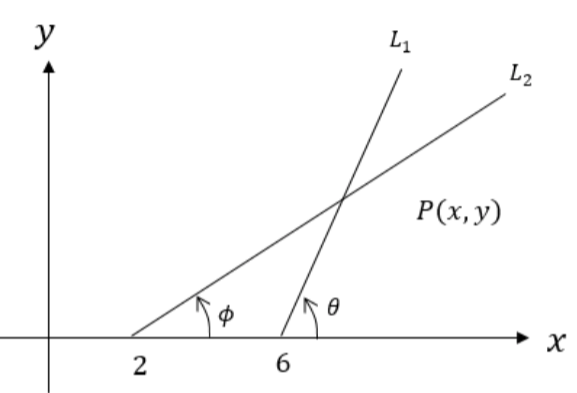
\includegraphics[width=0.25\linewidth]{images/t2w8q3a1.png}
    \end{figure}

    By the geometry rule 'exterior angle equals the sum of the two opposite interior angles', it follows that $\theta - \phi = \frac{\pi}{4}$ and that can be seen in the diagram as below:

    \begin{figure}[h]
        \centering
        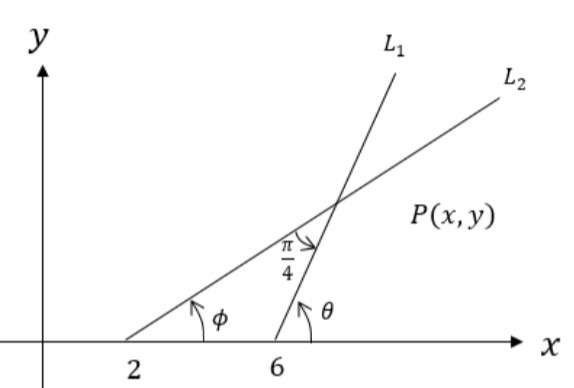
\includegraphics[width=0.25\linewidth]{images/t2w8q3a2.png}
    \end{figure}

    As the two angles $\theta$ and $\phi$ vary, but the $\frac{\pi}{4}$ is constant, $P$ forms an arc, based on the geometry rule 'angles on the same arc are equal'.

    \begin{figure}[h]
        \centering
        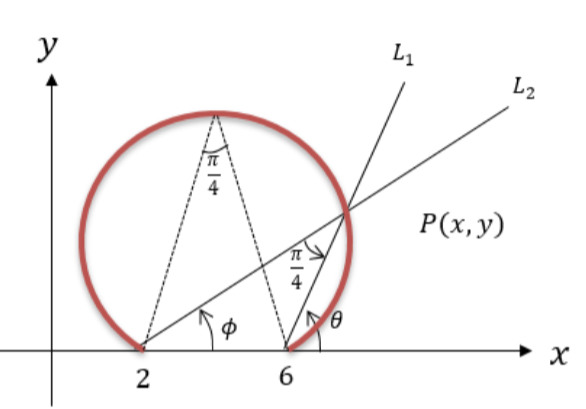
\includegraphics[width=0.25\linewidth]{images/t2w8q3a3.png}
    \end{figure}

    To find the centre of the circle (and hence the equation), we use the geometry rule 'angle at centre is twice the angle at the circumference'. This means the angle at the centre will be $\frac{\pi}{2}$. This triangle must be isosceles as two sides are radii.

    \begin{figure}[H]
        \centering
        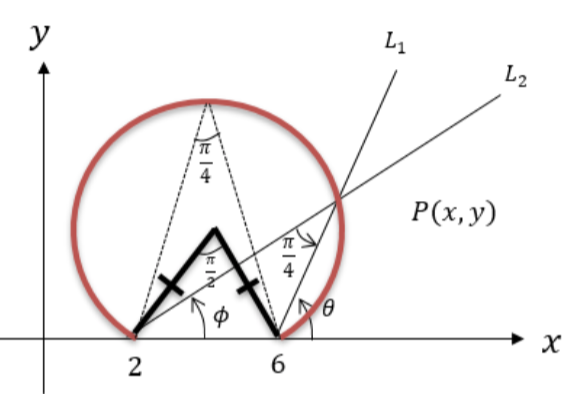
\includegraphics[width=0.25\linewidth]{images/t2w8q3a4.png}
    \end{figure}

    From here if we drop a perpendicular line down to create a right angle triangle it is simple enough to find the radius of the circle as $\sqrt{8}$:

    \begin{figure}[h]
        \centering
        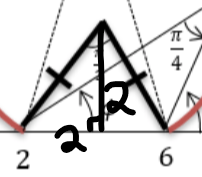
\includegraphics[width=0.15\linewidth]{images/t2w8q3a5.png}
    \end{figure}

    Since the centre lies on the line $x=4$, it means we have $(x-4)^2 + (y-b)^2 = 8$

    Substituting in one of the known points (2,0) or (6,0) we can find \textit{b}.

    $(2-4)^2+(-b)^2=8$

    $4+b^2=8$

    $b=2$

    So the equation is $(x-4)^2 + (y-2)^2 = 8$

    \item
    We know $\overline{\rm AB}$=6cm. 

    Adding a line from R to O, the centre of the small circle, we know $\overline{\rm OR}=2+r$, where r = the radius of the small circle.

    Forming a right-triangle by dropping a vertical line from the O and drawing a horizontal line from R, we can see the following:

    \begin{figure}[H]
        \centering
        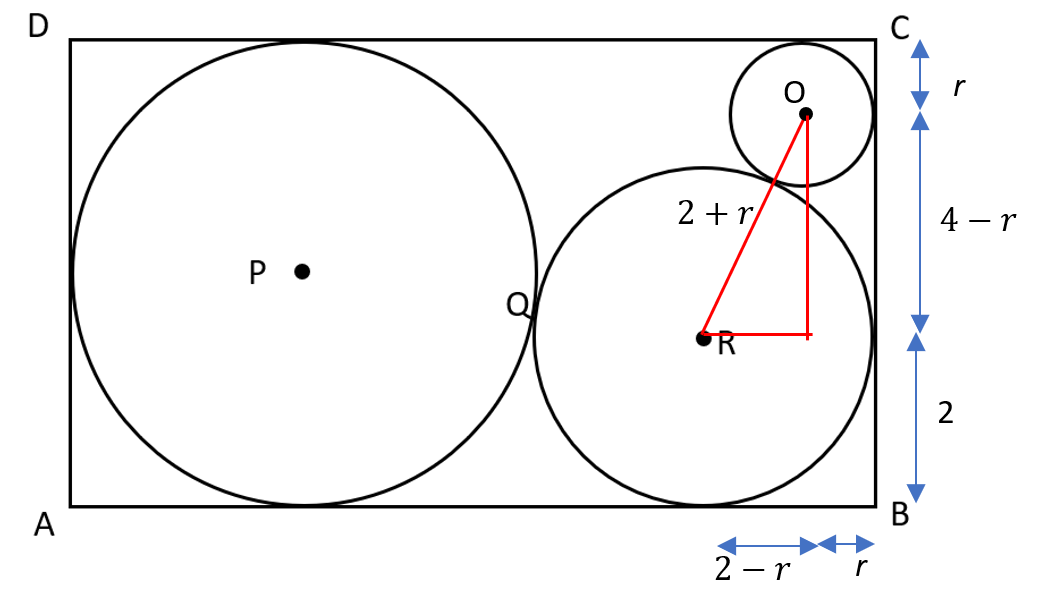
\includegraphics[width=0.6\linewidth]{images/t2w8q4a1.png}
    \end{figure}

    This gives us the following triangle:

    \begin{figure}[H]
        \centering
        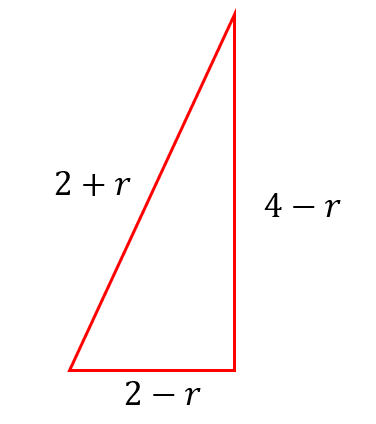
\includegraphics[width=0.25\linewidth]{images/t2w8q4a2.png}
    \end{figure}

    Using Pythagoras to solve for \textit{r}:

    $(2-r)^2+(4-r)^2=(2+r)^2$

    $4-4r+r^2+16-8r+r^2=4+4r+r^2$

    $2r^2-12r+20=r^2+4r+4$

    $r^2-16r+16=0$

    $r=8-4\sqrt{3}$

\end{enumerate}

\end{document}

